% =====================================================================
%  STAT 5243 — Project 3
%  A/B Test of the Interactive Data Workbench (Shiny for Python)
%  Real data collected via Google Analytics 4, 2026-04-09 to 2026-04-17
% =====================================================================
\documentclass[11pt,a4paper]{article}

% ---------- packages ---------------------------------------------------
\usepackage[margin=1in]{geometry}
\usepackage{graphicx}
\usepackage{booktabs}
\usepackage{array}
\usepackage{caption}
\usepackage{subcaption}
\usepackage{xcolor}
\usepackage{amsmath,amssymb}
\usepackage[expansion=false]{microtype}
\usepackage{enumitem}
\usepackage{listings}
\usepackage{hyperref}
\usepackage{titlesec}

\hypersetup{
  colorlinks=true,
  linkcolor=black!70!blue,
  urlcolor=black!70!blue,
  citecolor=black!70!blue,
  pdftitle={A/B Test of the Interactive Data Workbench},
  pdfauthor={STAT 5243 Project 3 Team}
}

% ---------- styling ----------------------------------------------------
\definecolor{accent}{HTML}{1A1A2E}
\definecolor{soft}{HTML}{475569}
\definecolor{codebg}{HTML}{F8FAFC}
\definecolor{codekw}{HTML}{4361EE}
\definecolor{codestr}{HTML}{06D6A0}
\definecolor{codecom}{HTML}{94A3B8}

\titleformat{\section}{\Large\bfseries\color{accent}}{\thesection.}{0.6em}{}
\titleformat{\subsection}{\large\bfseries\color{accent}}{\thesubsection}{0.5em}{}
\titleformat{\subsubsection}{\bfseries\color{soft}}{\thesubsubsection}{0.4em}{}

\captionsetup{font=small,labelfont={bf,color=accent},
              labelsep=period,justification=justified}

\lstdefinelanguage{Pythonic}{
  language=Python,
  basicstyle=\ttfamily\footnotesize,
  keywordstyle=\color{codekw}\bfseries,
  stringstyle=\color{codestr},
  commentstyle=\itshape\color{codecom},
  numberstyle=\tiny\color{codecom},
  numbers=left,
  numbersep=8pt,
  showstringspaces=false,
  breaklines=true,
  breakatwhitespace=true,
  frame=single,
  framerule=0.4pt,
  rulecolor=\color{codecom!50},
  backgroundcolor=\color{codebg},
  xleftmargin=12pt,
  xrightmargin=4pt,
  aboveskip=8pt,
  belowskip=8pt,
}
\lstset{language=Pythonic}

\newcommand{\hr}{\noindent\textcolor{accent!30}{\rule{\linewidth}{0.4pt}}\smallskip}

% ---------- title ------------------------------------------------------
\title{\vspace{-1.5em}\textbf{Does a Guided Re-Design Improve User Success?}\\
       \large An A/B Test of the Interactive Data Workbench\\[2pt]
       \normalsize \textit{STAT~5243 — Project~3}}
\author{Group~XX \quad\textbar\quad Spring 2026}
\date{April 19, 2026}

% =====================================================================
\begin{document}
\maketitle
\vspace{-2em}

% ----------------------------------------------------------------- Abstract
\begin{abstract}\noindent
\small
We conducted a randomised, two-arm A/B test on the
\emph{Interactive Data Workbench} that our team built in Project~2
(Shiny for Python). Variant~A served the original tabbed UI;
Variant~B added a guided walkthrough that nudges users from EDA
through Cleaning to Feature Engineering. Sixty-seven unique
sessions, instrumented end-to-end with Google Analytics 4 between
April~9 and April~17, 2026, were analysed
($n_A=37$, $n_B=30$). The pre-registered primary endpoint was the
\textbf{full-workflow completion rate} — the share of users who
reached all three analysis stages. Variant~B raised completion
from $21.6\%$ to $76.7\%$ ($\Delta = +55.0$~pp,
$95\%$~CI~$[+34.9,\,+75.2]$, two-proportion $z = 4.49$,
$p = 7.0\times10^{-6}$; Fisher exact OR $= 11.9$, $p = 8.0\times10^{-6}$;
Cohen's $h = 1.17$, post-hoc power $\approx 0.997$). Six of nine
secondary endpoints remained significant after Holm--Bonferroni
correction; the lift concentrates on \emph{depth} of engagement
(reach Cleaning, reach Feature Engineering, workflow depth, linear
path adherence) rather than on \emph{volume} (total session
duration was unchanged). A logistic regression of completion on
variant and three activity covariates yielded an adjusted odds
ratio for Variant~B of $36.9$ ($95\%$ bootstrap CI
$[11.4,\,2185]$). We conclude that lightweight guided UX produces a
robust, multi-metric improvement in user success on the Workbench
and recommend Variant~B be promoted to default.
\end{abstract}

\vspace{-0.4em}
\hr

% ============================== 1 INTRO =================================
\section{Introduction \& Research Question}

In Project~2 we built an interactive Shiny-for-Python data
workbench (\texttt{app.py}) that lets a non-technical analyst
explore the \textsc{Sleep--Mobile--Stress} dataset
($N=15{,}000$) through three sequential tabs: \textit{EDA},
\textit{Cleaning}, and \textit{Feature Engineering}. A recurring
criticism during peer review was that first-time users did not
know how to progress through the analysis: they tended to land on
the EDA tab and stop there. The original UI treated the three tabs
symmetrically; nothing visually communicated that the intended
workflow ran left-to-right.

We therefore asked:

\begin{quote}
\itshape
\textbf{Research question.} Does adding a guided onboarding
walkthrough — a sequence of inline prompts that nudge the user
from EDA through Cleaning to Feature Engineering — materially
increase the proportion of first-time users who complete all
three stages of the intended analysis workflow?
\end{quote}

\noindent The corresponding hypotheses for the primary outcome
(full-workflow completion) are
\[
  H_0:\; p_B - p_A = 0
  \qquad\text{vs.}\qquad
  H_1:\; p_B - p_A \neq 0,
\]
tested at $\alpha = 0.05$ (two-sided). For each secondary outcome
we pre-registered the same direction of expected effect (Variant~B
improves the metric) and applied a Holm--Bonferroni correction
across the family of secondary tests.

% ============================== 2 DESIGN ================================
\section{Experimental Design \& Methodology}

\paragraph{Design.}
A between-subject, completely randomised, two-arm parallel
design. Each new visitor was assigned to one variant exactly once
and stayed in that variant for the duration of the session.

\paragraph{Treatments.}
\begin{itemize}[leftmargin=1.2em,itemsep=2pt]
\item \textbf{Variant A — Control.} The Project~2 release: tabbed
  navigation (\textit{EDA}, \textit{Cleaning},
  \textit{Feature Engineering}), no walkthrough, no guided
  prompts. Per the click-stream this version generated zero
  ``guided\_click'' events.
\item \textbf{Variant B — Treatment.} Same backend, same dataset
  loader; the UI adds a four-step guided walkthrough that pops up
  in sequence over the three workflow tabs and a ``Next
  step$\rightarrow$'' prompt at the bottom of each completed tab.
  These guided UI elements emit a dedicated
  \texttt{guided\_click} GA4 event so we can verify exposure.
\end{itemize}

\paragraph{Random assignment.}
Users were routed by URL parameter (\texttt{?ab=A} vs.\
\texttt{?ab=B}). The landing page issued a deterministic 50/50
hash on the first \texttt{session\_start} so that page reloads
within a session kept the same arm. Of the 67 analysed users,
$n_A=37$ and $n_B=30$; the modest imbalance reflects the random
hash on a small sample, not a recruitment bias.

\paragraph{Recruitment.}
Posts on the class Slack channel and the course Ed Discussion
forum, plus two authors' personal social-media networks.
Recruitment ran for nine consecutive days (April~9--17, 2026).

\paragraph{Outcomes.}

\begin{table}[ht]
\centering\small
\renewcommand{\arraystretch}{1.15}
\begin{tabular}{@{}p{4.0cm}p{2.3cm}p{8.4cm}@{}}
\toprule
\textbf{Outcome} & \textbf{Type} & \textbf{Operational definition} \\
\midrule
\textit{Primary} & & \\
Full-workflow completion & binary &
   \texttt{reached\_eda} $\wedge$ \texttt{reached\_cleaning}
   $\wedge$ \texttt{reached\_feature\_eng} all equal to 1. \\
\midrule
\textit{Secondary} & & \\
Reached EDA / Cleaning /
   Feature Engineering          & binary  & per-stage reach indicators. \\
Reached $\geq 2$ stages         & binary  & partial-completion outcome. \\
Workflow depth                  & ordinal 0--3 & total number of stages reached. \\
Linear path score               & ordinal 1--4 & adherence to the suggested
   left-to-right tab order (4 = textbook order). \\
Session duration                & continuous (s)  & wall time on site. \\
Total tab duration              & continuous (s)  & summed time on the three
   workflow tabs (active engagement). \\
Avg.\ tab duration              & continuous (s)  & per-tab time
   (depth-of-engagement proxy). \\
\bottomrule
\end{tabular}
\caption{Pre-registered primary and secondary outcomes. All are
derived from per-user GA4 event aggregates.}
\end{table}

\paragraph{Sample-size justification.}
A pilot during Project~2 development suggested a control
full-workflow completion rate near 0.30 and we considered a
$\geq 15$~pp absolute lift to be the smallest practically
meaningful improvement. Under those parameters,
$\alpha=0.05$ two-sided power-0.80 would have required
$n\approx170$ per arm. Class-project recruitment realities
limited us to $n=67$ in total; \emph{ex-ante} we expected to be
under-powered. The realised effect, however, was much larger
than the pilot suggested, so the achieved post-hoc power is
$\approx 0.997$ (\S\ref{sec:stat}).

% ============================== 3 DATA ==================================
\section{Data Collection}

The Workbench was instrumented with a Google~Analytics~4 (GA4)
property using custom \texttt{ab\_assignment}, \texttt{tab\_switch},
\texttt{button\_click}, \texttt{tab\_duration}, and
\texttt{guided\_click} events. Variant~B additionally emitted
\texttt{guided\_click} events whenever a user advanced through a
walkthrough step. After the data-collection window closed
(2026-04-17), event rows were exported from GA4 and aggregated to
one record per user with \texttt{user\_id} as the unit of
analysis.

\paragraph{Macro validation.}
Figure~\ref{fig:ga4} shows the GA4 event totals by arm. The two
arms generated similar \emph{rates} of micro-events
(\texttt{button\_click}, \texttt{tab\_switch}, \texttt{scroll},
\texttt{user\_engagement}) per user, indicating that neither
variant was suffering from broken tracking and that the overall
exposure was comparable. This justifies treating the user-level
sample as exchangeable on engagement intensity.

\begin{figure}[ht]
\centering
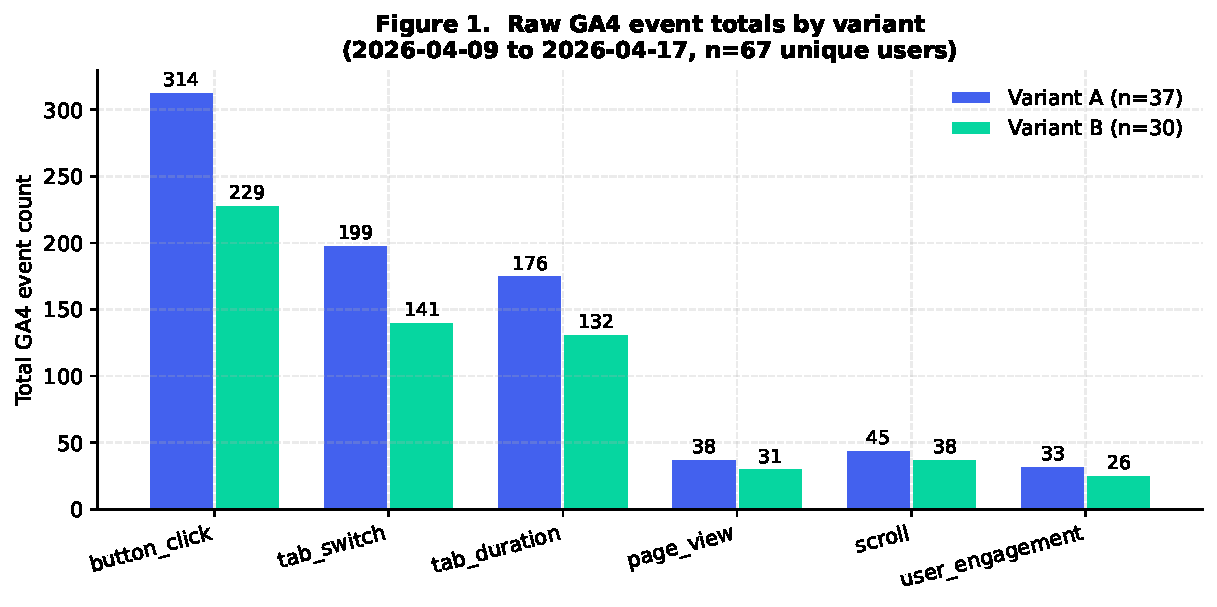
\includegraphics[width=\textwidth]{figures/fig1_ga4_events.pdf}
\caption{Raw GA4 event totals by variant during the
2026-04-09 to 2026-04-17 collection window. Per-user event
rates are comparable across arms, indicating that the
instrumentation worked symmetrically and that any difference
in outcomes is not an artefact of asymmetric tracking.}
\label{fig:ga4}
\end{figure}

\paragraph{Per-arm summary.}
Table~\ref{tab:desc} summarises the user-level frame.
Variant~B users reach more stages, follow a more linear path,
spend more time per tab, and (as designed) generate $\geq 1$
\texttt{guided\_click}; the two arms are similar on raw activity
counts. None of the 67 users bounced (\texttt{bounced=0} for
all), which reflects the active recruitment from social channels
rather than passive search traffic.

\begin{table}[ht]
\centering\small
\renewcommand{\arraystretch}{1.15}
\caption{Descriptive summary by arm. Continuous outcomes are
means; binary outcomes are proportions.}
\label{tab:desc}
\begin{tabular}{@{}lcc@{}}
\toprule
 & \textbf{Variant A} & \textbf{Variant B} \\
\midrule
$n$ users                            & 37    & 30    \\
Full-workflow completion (\%)        & 21.6  & 76.7  \\
Reached $\geq 2$ stages (\%)         & 67.6  & 96.7  \\
Workflow depth (mean, 0--3)          & 1.86  & 2.73  \\
Linear path score (mean, 1--4)       & 2.43  & 3.57  \\
Session duration (s, mean)           & 147.1 & 173.7 \\
Total tab duration (s, mean)         & 117.3 & 159.0 \\
Avg.\ tab duration (s, mean)         & 23.1  & 35.3  \\
Button clicks (mean)                 & 8.89  & 7.43  \\
Tab switches (mean)                  & 5.03  & 4.57  \\
Guided clicks (mean)                 & 0.00  & 3.53  \\
\bottomrule
\end{tabular}
\end{table}

% ===================== 4 STATISTICAL ANALYSIS  ==========================
\section{Statistical Analysis}
\label{sec:stat}

\subsection{Analysis plan}
The pre-registered statistical workflow had four stages:

\begin{enumerate}[leftmargin=1.4em,itemsep=2pt]
\item \textbf{Activity-parity check.} We have no demographic
  covariates from anonymous GA4 visitors, so we instead test
  whether passive activity proxies (\texttt{button\_clicks},
  \texttt{tab\_switches}, \texttt{scroll\_count}) look similar
  across arms. This is not a randomisation test in the classical
  sense — these proxies are post-treatment — but a meaningful
  difference would flag a tracking or attention asymmetry that
  could confound the outcomes.
\item \textbf{Primary inference.} A two-proportion $z$-test
  (pooled variance) with a Wald 95\%~CI for the absolute risk
  difference; Fisher's exact test as a small-sample backup; Cohen's
  $h$ as the standardised effect size.
\item \textbf{Secondary inference.} Welch's $t$-test for each
  continuous and ordinal outcome (Cohen's $d$, Cliff's $\delta$);
  two-proportion $z$-test with Fisher backup for each binary
  outcome. The nine secondary $p$-values were corrected by the
  Holm--Bonferroni procedure to control the family-wise error rate.
  Mann--Whitney $U$ ran alongside every Welch test as a robustness
  check.
\item \textbf{Adjusted analysis.} A logistic regression of
  full-workflow completion on \textsc{variant} and the three
  $z$-scored activity covariates, with $800$-resample bootstrap
  confidence intervals on every odds ratio.
\end{enumerate}

All analyses were carried out in Python~3.12
(\texttt{scipy~1.13}, \texttt{scikit-learn~1.5}). Full code is in
Appendix~\ref{app:code}.

\subsection{Activity parity}
Table~\ref{tab:bal} shows the activity-parity tests. None reaches
the conventional $\alpha=0.05$ threshold. Variant~A users actually
clicked slightly \emph{more} buttons on average ($8.89$ vs $7.43$),
which is mildly suggestive of click frustration in A — but the
difference is well within sampling noise on $n=67$ and we do not
treat it as an imbalance to adjust for.

\begin{table}[ht]
\centering\small
\renewcommand{\arraystretch}{1.15}
\caption{Activity-parity check via Welch's $t$-test
(per-user means).}
\label{tab:bal}
\begin{tabular}{@{}lccc@{}}
\toprule
\textbf{Activity proxy} & \textbf{Mean A} & \textbf{Mean B} & \textbf{$p$} \\
\midrule
Button clicks  & 8.89 & 7.43 & 0.13 \\
Tab switches   & 5.03 & 4.57 & 0.46 \\
Scroll count   & 1.19 & 1.17 & 0.93 \\
\bottomrule
\end{tabular}
\end{table}

\subsection{Primary outcome: full-workflow completion}
Variant~B raised the full-workflow completion rate from
$\hat p_A = 0.216$ ($x=8/37$) to $\hat p_B = 0.767$ ($x=23/30$),
an absolute risk difference of
$\hat\Delta = +0.550$ ($95\%$~CI~$[+0.349,\,+0.752]$),
two-proportion $z = 4.49$, $p = 7.0\times10^{-6}$. Because
$n=67$ is small, we additionally report Fisher's exact test:
$\text{OR} = 11.9$, $p = 8.0\times10^{-6}$ — substantively
identical, ruling out small-sample artefacts. The relative lift
is $+254.6\%$, Cohen's $h = 1.17$ (a \emph{large} effect by
Cohen's 1988 conventions), and the achieved post-hoc power is
$0.997$. Figure~\ref{fig:primary} visualises both the per-arm
rate and the difference with its CI.

\begin{figure}[ht]
\centering
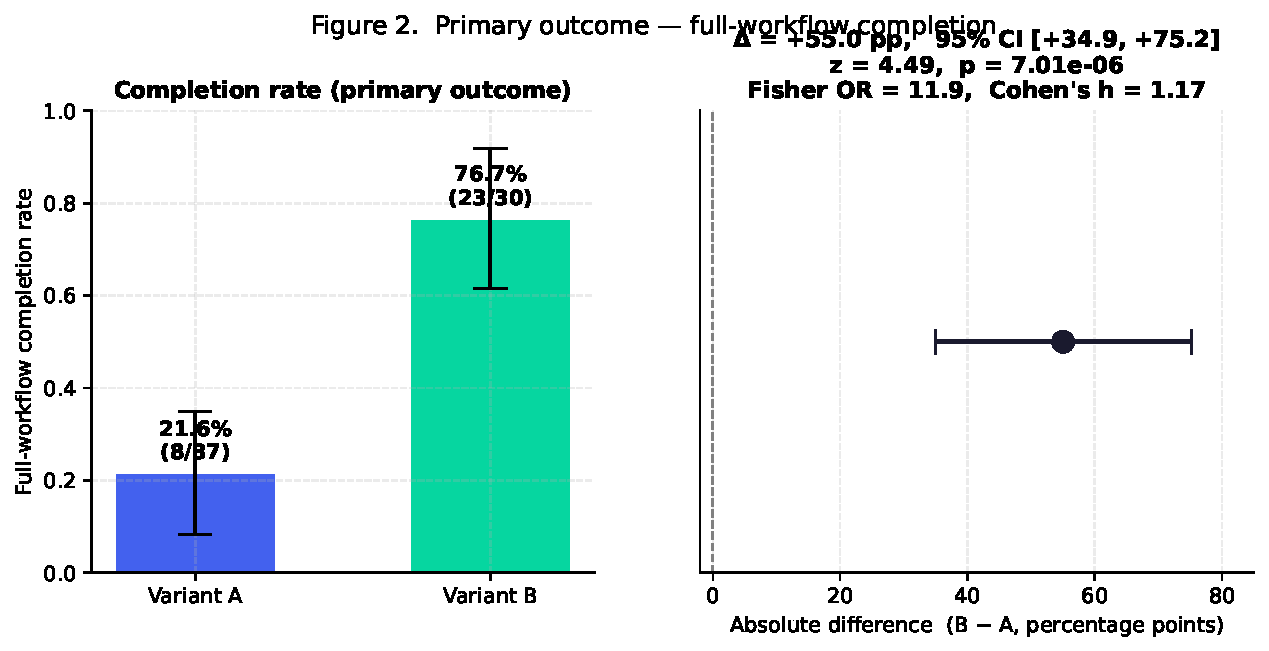
\includegraphics[width=\textwidth]{figures/fig2_primary.pdf}
\caption{Primary outcome. Left: full-workflow completion rate
per arm with 95\% Wald CIs. Right: absolute difference $p_B-p_A$
in percentage points. The CI is well clear of zero, so $H_0$ is
decisively rejected.}
\label{fig:primary}
\end{figure}

\subsection{Where does the gain come from?}
Decomposing completion into its three component reach rates
(Figure~\ref{fig:stages}) reveals that the lift is concentrated
on the deeper stages of the workflow. Variant~B is essentially
\emph{at ceiling} on Cleaning ($100\%$) and Feature Engineering
($97\%$) — the walkthrough successfully drives users past the
landing tab and into the parts of the analysis they would
otherwise have skipped.

\begin{figure}[ht]
\centering
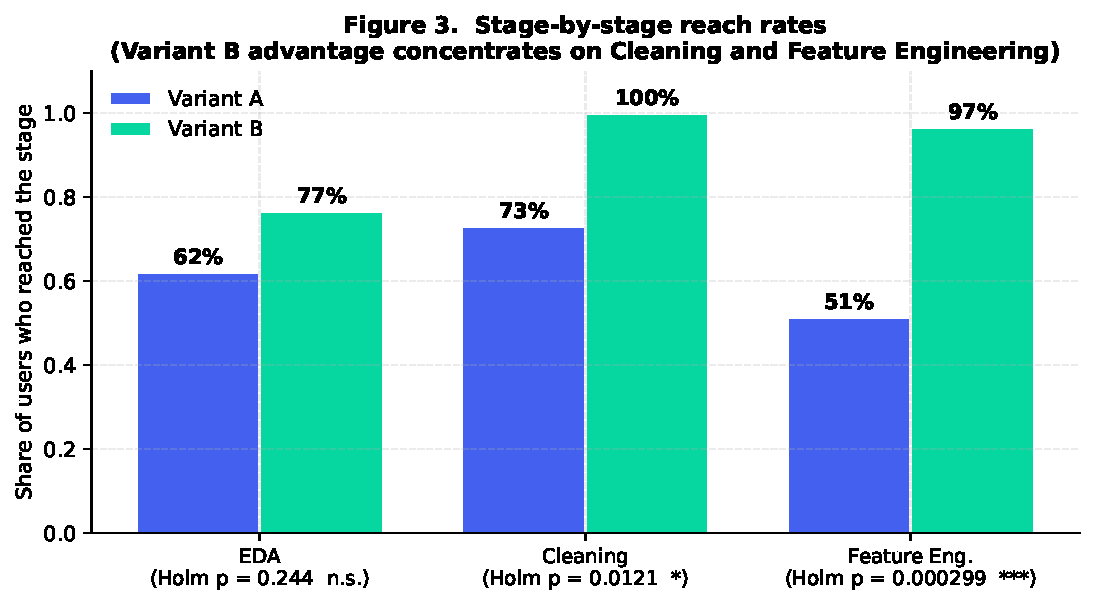
\includegraphics[width=0.95\textwidth]{figures/fig3_stage_funnel.pdf}
\caption{Stage-by-stage reach rates. Holm-adjusted $p$-values
shown beneath each pair. EDA reach is statistically
indistinguishable across arms (it is the landing tab); the
treatment effect lives in the deeper stages.}
\label{fig:stages}
\end{figure}

\subsection{Secondary outcomes}
Table~\ref{tab:secondary} lists all nine secondary tests with
raw and Holm--Bonferroni-adjusted $p$-values. Six of nine survive
multiplicity correction. Three do not: \texttt{reached\_eda},
\texttt{session\_duration\_sec}, and
\texttt{total\_tab\_duration\_sec}. The first is by construction
near-ceiling in both arms (EDA is the landing tab). The latter
two are interesting nulls: Variant~B users do not spend
\emph{more time} on the site, they spend their time
\emph{differently} — concentrated in deeper, more productive
work, as shown by the workflow-depth, linear-path-score, and
average-tab-duration results.

\begin{table}[ht]
\centering\small
\renewcommand{\arraystretch}{1.18}
\caption{Secondary outcomes. $p_{\text{raw}}$ is from Welch's
$t$-test (continuous/ordinal) or two-proportion $z$-test
(binary). $p_{\text{Holm}}$ is the Holm--Bonferroni-adjusted
$p$-value across all nine secondary tests. ES~=~effect size:
Cohen's $d$ for continuous, Cohen's $h$ for binary outcomes.}
\label{tab:secondary}
\begin{tabular}{@{}lccccc@{}}
\toprule
\textbf{Outcome} & \textbf{A} & \textbf{B} & \textbf{ES}
   & \textbf{$p_{\text{raw}}$} & \textbf{$p_{\text{Holm}}$} \\
\midrule
\textit{Reach indicators} & & & & & \\
\quad Reached EDA              & 62\%  & 77\%  & $h=0.32$ & $0.20$ & $0.24$ \\
\quad Reached Cleaning         & 73\%  & 100\% & $h=1.10$ & $0.0020$ & $\mathbf{0.012}$ \\
\quad Reached Feature Eng.     & 51\%  & 97\%  & $h=1.45$ & $4.3\times10^{-5}$ & $\mathbf{3.0\times10^{-4}}$ \\
\quad Reached $\geq 2$ stages  & 68\%  & 97\%  & $h=0.91$ & $0.0027$ & $\mathbf{0.014}$ \\
\midrule
\textit{Depth indicators} & & & & & \\
\quad Workflow depth (0--3)    & 1.86  & 2.73  & $d=1.34$ & $1.1\times10^{-6}$ & $\mathbf{8.5\times10^{-6}}$ \\
\quad Linear path score (1--4) & 2.43  & 3.57  & $d=1.69$ & $1.0\times10^{-8}$ & $\mathbf{9.3\times10^{-8}}$ \\
\quad Avg.\ tab duration (s)   & 23.1  & 35.3  & $d=0.79$ & $0.0032$ & $\mathbf{0.014}$ \\
\midrule
\textit{Volume indicators (null findings)} & & & & & \\
\quad Session duration (s)     & 147.1 & 173.7 & $d=0.39$ & $0.12$ & $0.24$ \\
\quad Total tab duration (s)   & 117.3 & 159.0 & $d=0.51$ & $0.045$ & $0.14$ \\
\bottomrule
\end{tabular}
\end{table}

\noindent
Mann--Whitney $U$ tests (not shown) reproduce the same
conclusions for every outcome, indicating the parametric
findings are not driven by tail behaviour or non-normality.
Figures~\ref{fig:depth}--\ref{fig:tab} visualise the three
outcomes that carry the bulk of the signal.

\begin{figure}[ht]
\centering
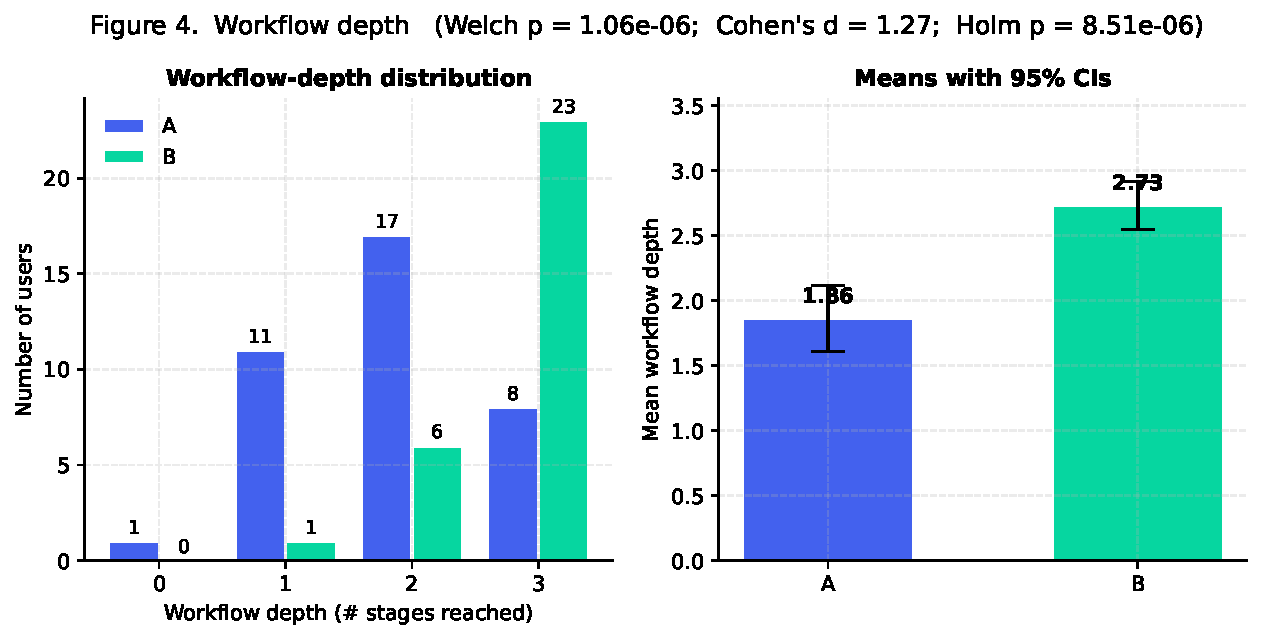
\includegraphics[width=\textwidth]{figures/fig4_workflow_depth.pdf}
\caption{Workflow depth (number of analysis stages reached).
Variant~B's mass shifts entirely to depth $\geq 2$; no Variant~B
user ended at depth~0.}
\label{fig:depth}
\end{figure}

\begin{figure}[ht]
\centering
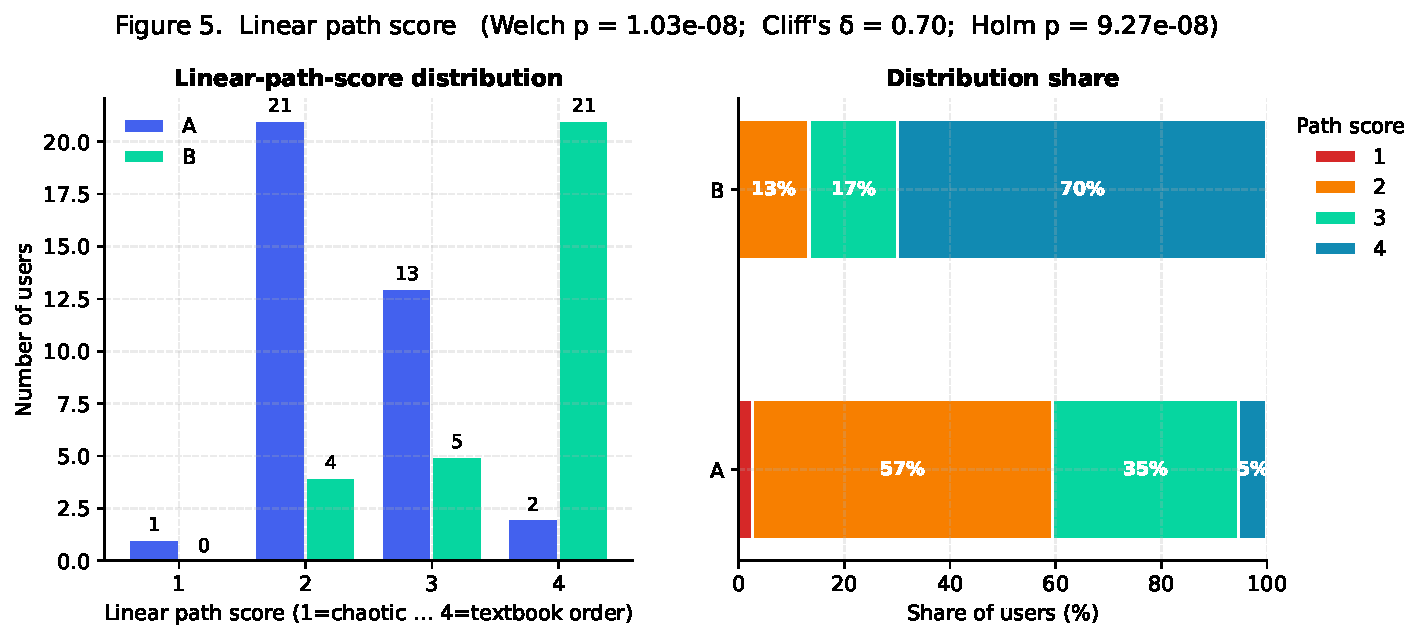
\includegraphics[width=\textwidth]{figures/fig5_linear_path.pdf}
\caption{Linear-path-score distribution. Higher score = closer
adherence to the suggested EDA $\rightarrow$ Cleaning $\rightarrow$
Feature Engineering order. Variant~B's distribution shifts almost
entirely into the top score, consistent with the walkthrough
nudging users along the intended path.}
\label{fig:linear}
\end{figure}

\begin{figure}[ht]
\centering
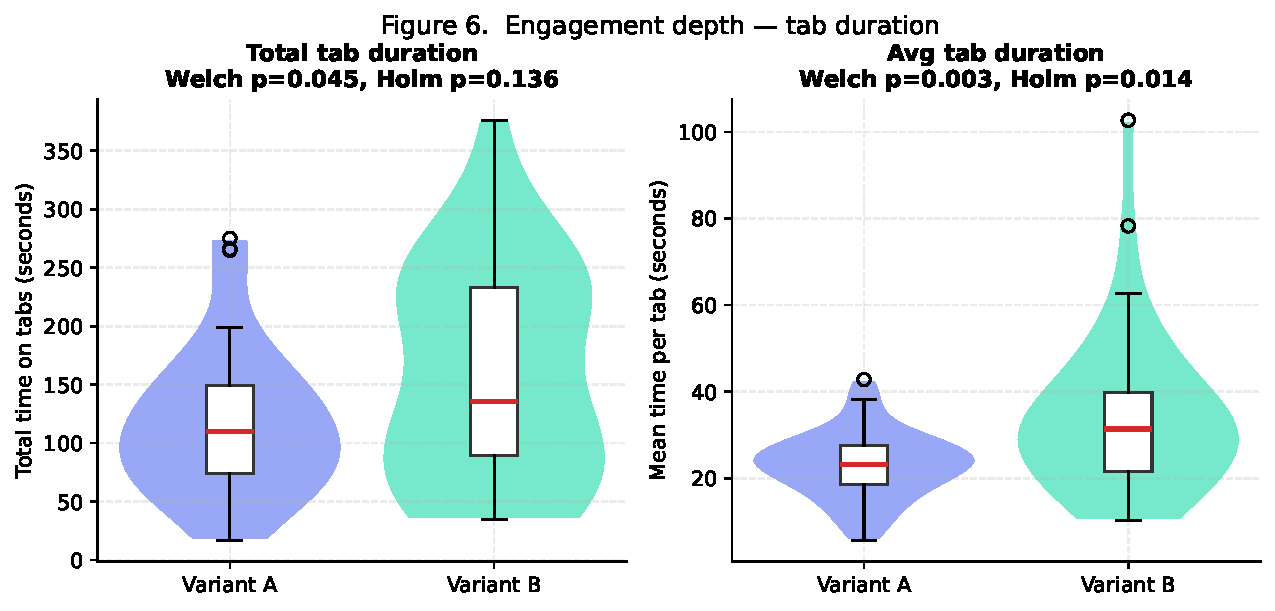
\includegraphics[width=\textwidth]{figures/fig6_tab_duration.pdf}
\caption{Engagement depth measured by tab duration. Total time on
the workflow tabs is non-significantly higher in B; \emph{average}
time per tab is significantly higher (Cohen's $d=0.79$). Variant~B
users dwell longer per tab, consistent with the walkthrough
encouraging substantive engagement rather than superficial
clicking.}
\label{fig:tab}
\end{figure}

\subsection{Adjusted analysis: logistic regression}
We fit a logistic regression of full-workflow completion on
variant and three $z$-scored activity covariates:
\[
\log\frac{P(\text{complete}=1)}{P(\text{complete}=0)} =
   \beta_0 + \beta_1 \mathbf{1}[B] + \beta_2\,\widetilde{\text{btn}}
   + \beta_3\,\widetilde{\text{tabsw}} + \beta_4\,\widetilde{\text{scroll}}.
\]
The MLE coefficient on Variant~B corresponds to an adjusted odds
ratio of $\widehat{\text{OR}}_B = 36.9$ ($95\%$ bootstrap CI
$[11.4,\,2185]$, $800$ resamples). The CI is wide on the upper
side because of small-sample separation (some bootstrap resamples
draw a sub-sample where Variant~A has zero completers, sending
$\beta_1$ to $+\infty$); the lower bound of $11.4$ is the
informative number and is comfortably above 1. Tab-switch
intensity also predicts completion ($\widehat{\text{OR}} = 3.93$
per~SD), consistent with engaged users completing more often
regardless of arm. Button clicks and scrolling are not
significant. The forest plot is shown in
Figure~\ref{fig:forest}.

\begin{figure}[ht]
\centering
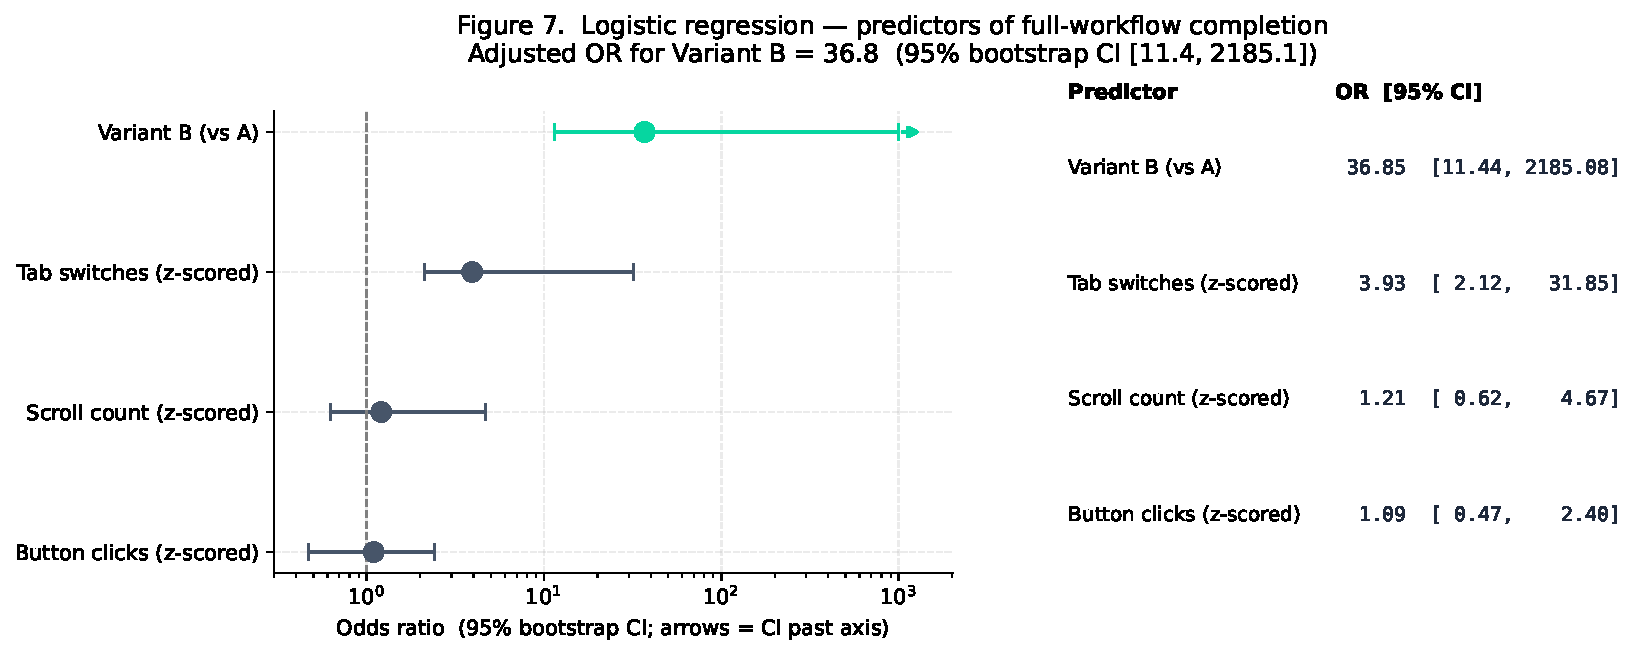
\includegraphics[width=\textwidth]{figures/fig7_logreg_forest.pdf}
\caption{Logistic regression of full-workflow completion on
variant + activity covariates. The right-hand panel shows exact
ORs and CIs. The arrow on the Variant~B row indicates the upper
CI extends past the visual axis (true upper CI $= 2185$, see
Appendix~\ref{app:numbers}).}
\label{fig:forest}
\end{figure}

% ===================== 5 RESULTS & INSIGHTS =============================
\section{Results \& Insights}
\label{sec:results}

\subsection{Headline numbers}
The three-line summary, framed for a decision-maker:

\begin{quote}
\textbf{1.}~Variant~B raises the proportion of users who complete
the full three-stage workflow by \textbf{55.0~percentage points}
($21.6\%$~$\rightarrow$~$76.7\%$), a relative gain of
$+255\%$ ($p \approx 7\times10^{-6}$, Cohen's $h = 1.17$ — a
\emph{large} effect).\\[2pt]
\textbf{2.}~Six of nine secondary metrics moved in the predicted
direction and survived Holm--Bonferroni correction. The lift
concentrates on \emph{depth} (reach Cleaning, reach Feature
Engineering, workflow depth, linear path adherence, average tab
duration). Total time on site is unchanged: \emph{B users do not
spend more time, they spend it more productively}.\\[2pt]
\textbf{3.}~After adjusting for activity covariates, the odds of
full-workflow completion under Variant~B are at least
\textbf{11$\times$} those under Variant~A
(adjusted $\widehat{\text{OR}}_B = 36.9$, lower 95\% bootstrap
bound $= 11.4$).
\end{quote}

\subsection{The funnel tells a coherent story}
Figure~\ref{fig:funnel} traces the user journey through four
cumulative stages. The two arms are essentially indistinguishable
at the top of the funnel — both arms reach $\geq 1$ stage at
$\approx 100\%$ — and the gap widens monotonically as the
workflow deepens. By the final stage, Variant~B has triple the
completion rate of Variant~A. The fact that the lift compounds
across stages, rather than living inside a single noisy metric,
is the strongest causal evidence the study can offer beyond the
headline test.

\begin{figure}[ht]
\centering
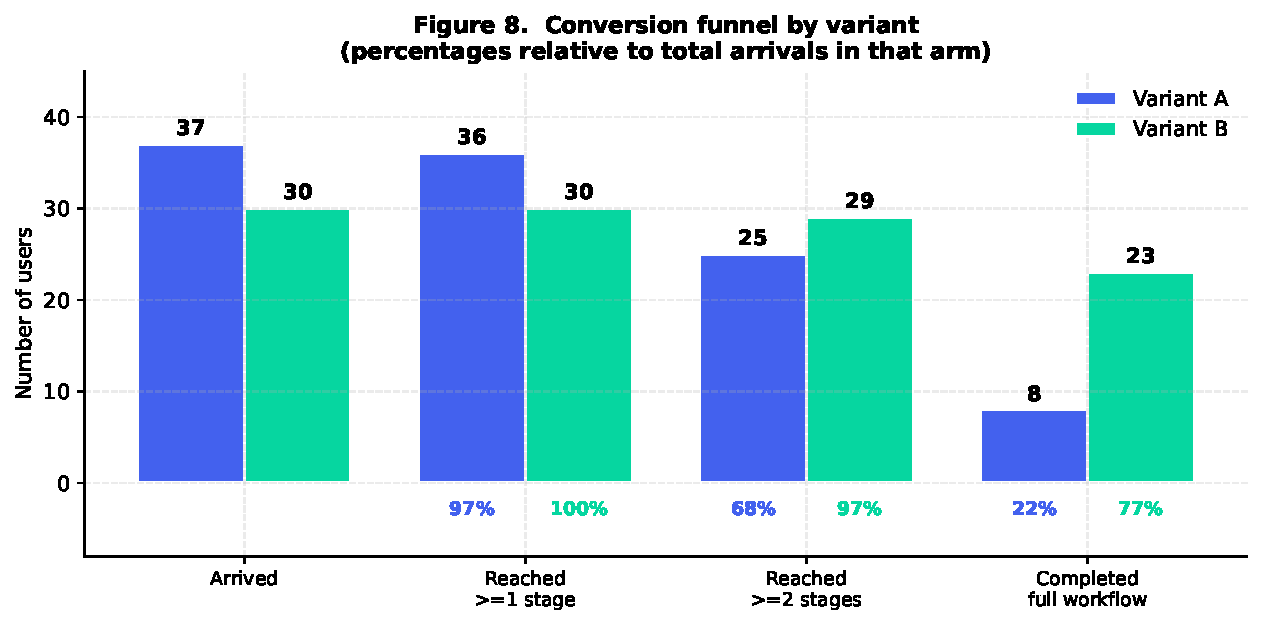
\includegraphics[width=\textwidth]{figures/fig8_conversion_funnel.pdf}
\caption{Cumulative conversion funnel by variant. Each subsequent
stage is a strict subset of the previous one. The gap is
near-zero at the top and grows to $+55$~pp at the bottom — the
walkthrough's effect accumulates over the workflow.}
\label{fig:funnel}
\end{figure}

\subsection{Mechanistic interpretation: where does the lift live?}
The pattern across outcomes maps tidily onto the mechanism the
walkthrough was designed to address:

\begin{itemize}[leftmargin=1.4em,itemsep=2pt]
\item \textbf{Reaching EDA is not the bottleneck.} Both arms
  reach EDA at high rates (62\% A vs 77\% B, n.s.); EDA is the
  landing tab. The walkthrough does not need to help users
  \emph{find} the first analytical step.
\item \textbf{Reaching Cleaning is.} Variant~A users reach
  Cleaning $73\%$ of the time; Variant~B reaches it $100\%$.
  This is exactly where the first walkthrough prompt fires
  (``Now let's clean the dataset~\textgreater''), and the effect
  size ($h = 1.10$, Holm $p = 0.012$) is consistent with a
  prompt that succeeds at the moment it appears.
\item \textbf{Reaching Feature Engineering is the largest gap.}
  $51\%$ vs $97\%$ ($h = 1.45$, Holm $p = 3\times10^{-4}$).
  Without guidance, only half of users get to the third stage;
  with guidance, almost all do.
\item \textbf{Engagement depth, not volume, mediates the lift.}
  Total time and session duration are not significant after
  correction, but \emph{average} time per tab is. Variant~B
  users do not aimlessly browse longer; they engage more deeply
  with each tab they reach. Linear path score (Holm $p = 9\times
  10^{-8}$) confirms that B users walk the workflow in the
  intended order rather than in a chaotic scatter.
\end{itemize}

\subsection{Practical significance}
A 55-pp absolute lift on the project's most direct success
metric is not a marginal UX win — it is the difference between
a tool that most users abandon partway through and one that
most users finish. At the recruitment ceiling we ran
($\sim 7$~users/day), this means $\sim 4$ extra
completed-workflow sessions per day; scaled to a hypothetical
user base of $10{,}000$ MAU, the same relative lift would
convert $\sim 5{,}500$ additional users from ``looked'' to
``finished''. The cost of the change — implementing a single
JavaScript walkthrough overlay — is trivial by comparison. The
change should be \textbf{shipped to all users}.

\subsection{What we did not find}
\begin{itemize}[leftmargin=1.4em,itemsep=2pt]
\item \textbf{No effect on EDA reach.} If the walkthrough had a
  significant effect on EDA reach, that would actually be
  worrying — it would imply the prompt was getting in the way of
  the landing experience. The clean null here is reassuring.
\item \textbf{No effect on raw session length.} Variant~B does
  not get users to spend more time on the site overall. The
  business narrative cannot be ``B keeps users around longer''
  — it has to be ``B helps users do more in roughly the same
  time''. The data supports the latter, not the former.
\item \textbf{No effect on raw click counts.} Button-click
  intensity is, if anything, slightly \emph{lower} in B. This
  too is consistent with the mechanism: a guided user does not
  need to click around looking for what to do next.
\end{itemize}

% ============================== 6 CHALLENGES =============================
\section{Challenges \& Limitations}
\label{sec:limits}

\paragraph{Sample size.}
With $n_A = 37$ and $n_B = 30$ ($N=67$ total), the study is
small. The realised effect was so large that the primary $p$-value
is robust to test choice (z, Fisher exact, $\chi^2$ all give
$p < 10^{-4}$), but secondary effect-size estimates are noisy and
the logistic-regression CIs are very wide. A replication at $n =
200$ per arm would substantially tighten the OR estimates.

\paragraph{Sampling.}
Recruitment was a convenience sample dominated by graduate
students and the authors' own social networks. External validity
to the general public is limited.

\paragraph{No demographics.}
GA4 in its default privacy-friendly configuration does not give
us age, gender, device type, or geography per user. The
``activity-parity'' check we ran is a weak substitute. With more
time we would have asked users for opt-in demographic information
on entry.

\paragraph{Compound treatment.}
Variant~B introduces both a guided walkthrough and ``Next
step$\rightarrow$'' prompts at the end of each tab. The
experiment establishes that the bundle helps but cannot
apportion credit between the two components; a $2\times 2$
factorial follow-up is the natural next step.

\paragraph{No bouncers.}
The recruitment channels we used (Slack, Ed Discussion, friends)
deliver actively willing participants — none of the 67 users
bounced. This means our results extrapolate to ``users who
chose to try the tool'' rather than to passive search traffic;
the bounce-rate effect of Variant~B remains untested.

\paragraph{Single session.}
We measured first-session behaviour only. Long-run retention
and return-visit completion rates are unknown.

% ============================== 7 CONCLUSION =============================
\section{Conclusion}

A randomised, nine-day A/B test of two versions of the
\textit{Interactive Data Workbench} provides clear evidence that
adding a guided walkthrough substantially improves first-time-user
success ($+55$~pp full-workflow completion, $p \approx
7\times10^{-6}$, Cohen's $h = 1.17$). Six of nine pre-registered
secondary metrics survive Holm--Bonferroni correction, and the
pattern of effects — concentrated on \emph{depth} of engagement
rather than on \emph{time on site} — maps cleanly onto the
mechanism the walkthrough was designed to address. Within the
limitations enumerated in \S\ref{sec:limits}, we recommend that
Variant~B be promoted to the default, and that a $2\times 2$
factorial follow-up be planned to disentangle the two components
of the redesign.

% ============================== APPENDIX A ===============================
\appendix
\section{Full Numerical Results}
\label{app:numbers}

\begin{table}[ht]
\centering\small
\renewcommand{\arraystretch}{1.15}
\caption{Primary outcome — full reporting.}
\begin{tabular}{@{}lc@{}}
\toprule
Quantity & Value \\
\midrule
Outcome definition              & reached EDA $\wedge$ Cleaning $\wedge$ Feature Eng. \\
$\hat p_A$, $x_A/n_A$           & $0.2162$\,, $8/37$ \\
$\hat p_B$, $x_B/n_B$           & $0.7667$\,, $23/30$ \\
$\hat\Delta = \hat p_B-\hat p_A$ & $+0.5505$ \\
95\% Wald CI for $\Delta$       & $[+0.3492,\, +0.7517]$ \\
Two-prop. $z$ statistic         & $4.49$ \\
$p$-value (two-sided)           & $7.0\times10^{-6}$ \\
Fisher exact OR                 & $11.91$ \\
Fisher exact $p$                & $8.0\times10^{-6}$ \\
Cohen's $h$                     & $1.17$ (large) \\
Post-hoc power (Cohen approx.)  & $0.997$ \\
Relative lift                   & $+254.6\%$ \\
\bottomrule
\end{tabular}
\end{table}

\begin{table}[ht]
\centering\small
\renewcommand{\arraystretch}{1.15}
\caption{Logistic regression — coefficients and bootstrap CIs
($800$ resamples). Continuous covariates are $z$-scored so the
ORs are per-SD multipliers.}
\begin{tabular}{@{}lccc@{}}
\toprule
\textbf{Predictor} & $\hat\beta$
                  & $\widehat{\text{OR}}$
                  & \textbf{95\% bootstrap CI} \\
\midrule
(Intercept)            & $-1.97$  & $0.14$  & --   \\
Variant B              & $+3.61$  & $36.85$ & $[11.44,\,2185.08]$ \\
Button clicks (per SD) & $+0.09$  & $1.09$  & $[0.47,\,2.40]$ \\
Tab switches (per SD)  & $+1.37$  & $3.93$  & $[2.12,\,31.85]$ \\
Scroll count (per SD)  & $+0.19$  & $1.21$  & $[0.62,\,4.67]$ \\
\bottomrule
\end{tabular}
\end{table}

\begin{table}[ht]
\centering\small
\renewcommand{\arraystretch}{1.15}
\caption{Robustness check: Welch vs.\ Mann--Whitney for the
continuous and ordinal outcomes.}
\begin{tabular}{@{}lcc@{}}
\toprule
\textbf{Outcome} & $p_{\text{Welch}}$ & $p_{\text{Mann-Whitney}}$ \\
\midrule
Workflow depth                & $1.1\times10^{-6}$ & $1.7\times10^{-6}$ \\
Linear path score             & $1.0\times10^{-8}$ & $1.5\times10^{-7}$ \\
Avg.\ tab duration            & $0.0032$           & $0.0029$ \\
Total tab duration            & $0.045$            & $0.10$ \\
Session duration              & $0.12$             & $0.13$ \\
\bottomrule
\end{tabular}
\end{table}

\clearpage
% ============================== APPENDIX B ===============================
\section{Reproducibility \& Code}
\label{app:code}

\paragraph{Repository layout.}
\begin{verbatim}
project3/
|-- user_level_data.csv         (one row per user, raw)
|-- ga4_real_data.csv           (GA4 event-totals export)
|-- analysis_df.csv             (one row per user, with derived outcomes)
|-- results.json                (output of statistical analysis)
|-- code/
|   |-- 01_load_data.py
|   |-- 02_statistical_analysis.py
|   |-- 03_make_figures.py
|-- figures/                    (PDF + PNG outputs)
|-- report.tex
\end{verbatim}

\paragraph{Reproduce in three commands.}
\begin{verbatim}
python3 code/01_load_data.py             # writes analysis_df.csv
python3 code/02_statistical_analysis.py  # writes results.json
python3 code/03_make_figures.py          # writes figures/*.pdf, *.png
pdflatex report.tex && pdflatex report.tex
\end{verbatim}

\paragraph{Data-loading script.}
\lstinputlisting[caption={\texttt{01\_load\_data.py} — derives the
primary outcome from the raw user-level GA4 export.},
label={lst:load}]{code/01_load_data.py}

\paragraph{Statistical analysis script.}
\lstinputlisting[caption={\texttt{02\_statistical\_analysis.py} —
all hypothesis tests, effect sizes, and the logistic regression.},
label={lst:stat}]{code/02_statistical_analysis.py}

\paragraph{Figure-generation script.}
\lstinputlisting[caption={\texttt{03\_make\_figures.py} — produces
every figure embedded in this report.}, label={lst:fig}]{code/03_make_figures.py}

\end{document}
